%
% Abschlussarbeit mit LaTeX
% ===========================================================================
% This is part of the book "Abschlussarbeit mit LaTeX".
% Copyright (c) 2002-2005 Tobias Erbsland, Andreas Nitsch
% See the file abschlussarbeit_mit_latex.tex for copying conditions.
%

\chapter{Grundlagen}
\label{sec:grundlagen}
\index{Grundlagen|(}

\DMLLaTeX{} ist einfacher zu erlernen, als du vielleicht denkst. Anders als grafische Tools, welche WYSIWYG\footnote{What You See Is What You Get} bieten (wollen), beschreibst du ähnlich wie bei HTML die Struktur deines Dokuments in einer speziellen Sprache. Danach \enquote{kompilierst} du das Dokument und erzeugst dadurch das fertige Dokument, zum Beispiel eine PDF-Datei.


\section{Das erste kleine LaTeX"=Dokument}

\subsection{Erstellen eines neuen Projekts}
\label{sec:erstellenneuesprojekt}
\index{Erstellen!Projekt}\index{Projekt erstellen}\index{Neues Projekt}

Starte jetzt im TeXnicCenter ein neues Projekt. Dazu gehst du auf \enquote{Datei}, dort auf \enquote{Neues Projekt...} (siehe dazu \cref{fig:beispiel1_01}).

\begin{figure}[ht]
	\begin{center}
		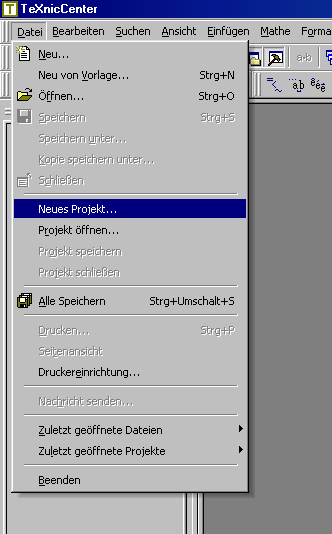
\includegraphics[width=3cm]{images/beispiel1_01.png}
	\end{center}
	\caption{Auswählen von \enquote{Neues Projekt...} über das Menü}
	\label{fig:beispiel1_01}
\end{figure}


Ein Dialogfenster öffnet sich, in dem du den Projekttyp\index{Projekttyp} auswählen kannst. Es steht nur \enquote{Leeres Projekt} zur Verfügung. Klicke dieses Icon an und wähle rechts das Basisverzeichnis aus. Für jedes \DMLLaTeX"=Dokument wird ein neues Unterverzeichnis in diesem Basisverzeichnis erstellt.

Ich empfehle dir Folgendes: Lege auf deinem Datenlaufwerk (z.\,B. M:\textbackslash ) ein Verzeichnis \enquote{Dokumente} an. Darin erstellst du z.\,B. noch ein Unterverzeichnis \enquote{LaTeX}.

Gib dieses Verzeichnis nun als \enquote{Basisverzeichnis} im Projektdialog an.

Jetzt kannst du einen Projektnamen eingeben. Gib z.\,B. \enquote{Beispiel1} als Projektnamen ein. Während du den Projektnamen eingibst, siehst du, dass das Basisverzeichnis im unteren Feld um diesen Projektnamen erweitert wird. Siehe dazu \cref{fig:beispiel1_02}.

\begin{figure}[ht]
	\begin{center}
		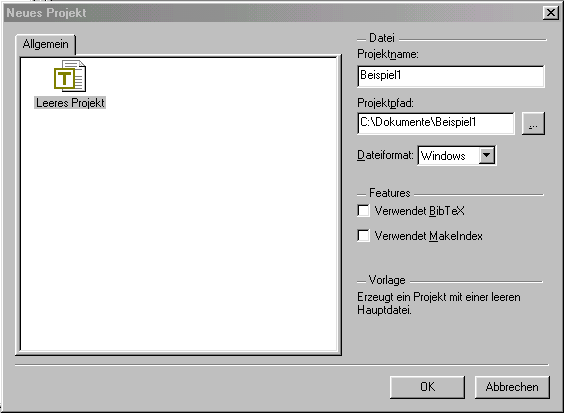
\includegraphics[width=5cm]{images/beispiel1_02.png}
	\end{center}
	\caption{Der Dialog für ein neues Projekt}
	\label{fig:beispiel1_02}
\end{figure}

Wenn du den Projektnamen eingegeben hast, klickst du auf \enquote{Ok}. Jetzt wird das neue Projekt erstellt. Dazu wird das Unterverzeichnis \enquote{Beispiel1} erstellt, und darin die Datei \enquote{Beispiel1.tcp}. Dies ist die Projektdatei.

Weiter wird eine neue Datei \enquote{Beispiel1.tex} erstellt. Dies ist unsere \DMLLaTeX"=Datei.

\subsection{Erstes Beispiel}
\label{sec:erstesbeispiel}

Schreibe jetzt folgende Zeilen in die leere Datei:

\lstinputlisting[caption=Beispiel1.tex, label=lst:beispiel01, frame=tb]%
	{listings/beispiel01.tex}

Die Zeilen 5--11 sind der Kopfbereich der Datei. Hier definieren wir Folgendes:

\begin{description}
\item[Zeile 5] Der Befehl \texttt{\textbackslash documentclass}\index{documentclass@\texttt{\textbackslash documentclass}} definiert unsere Dokumentklasse\index{Dokumentklasse}. Wir verwenden hier die Klasse \enquote{scrartcl}, welche für kleinere Artikel gedacht ist. Neben der \KOMAScript{} Klasse \enquote{scrartcl} gibt es z.\,B. noch \enquote{scrbook}, \enquote{scrreprt}, \enquote{scrlettr} und andere weniger übliche.
\item[Zeile 6] Mit dem Paket \enquote{ngerman}\index{Paket!ngerman}, welches wir hier laden, werden verschiedene Titel ins Deutsche übersetzt. So z.\,B. \enquote{Table of Contents} in \enquote{Inhaltsverzeichnis}. Zudem aktiviert dieses Paket die korrekte Silbentrennung für die neue deutsche Rechtschreibung.

Falls du lieber die alte deutsche Rechtschreibung verwenden möchtest, dann solltest du statt dem Paket \enquote{ngerman} das Paket \enquote{german}\index{Paket!german} einbinden.
\item[Zeile 7] \enquote{inputenc}\index{Paket!inputenc} binden wir ein, damit die deutschen Zeichen ä, ö, ü, Ä, Ö, Ü und ß automatisch erkannt werden und wir diese nicht als \enquote{''a} usw. schreiben müssen.
\item[Zeile 8] Das Paket \enquote{fontenc} mit der Option \enquote{T1}, ändert die Fontkodierung auf das \enquote{T1} Format. %TODO: Erläuterung, wozu dieses gut sein soll

Normalerweise verwendet \DMLLaTeX{} Schriftarten mit einem Umfang von 128 Zeichen. Darin sind z.\,B. keine Umlaute oder Buchstaben mit Akzenten enthalten. Diese werden jeweils aus dem Buchstaben und Akzent zusammengesetzt. Also \enquote{a} und \enquote{\textasciicircum} ergibt \enquote{â}.

Mittlerweile stehen für die meisten Schriften in den \DMLLaTeX"=Distributionen erweiterte \enquote{europäische} Versionen zur Verfügung (In der \enquote{T1-Codierung}). Diese Schriften enthalten bis zu 256 Zeichen. Dort sind auch Umlaute und akzentuierte Zeichen vorgefertigt enthalten. Das führt zu einer höheren typographischen Qualität der Dokumente und löst auch einige Probleme mit der Silbentrennung.
\item[Zeile 10 und 11] Hier definieren wir den Titel\index{Dokumenttitel} und den Autor\index{Autor} des Dokuments.
\end{description}

Die Zeilen 13--23 bilden dann den eigentlichen Inhalt des Dokuments. Der Dokumentinhalt wird immer durch die Zeilen \enquote{\textbackslash begin\{document\}} und \enquote{\textbackslash end\{document\}} eingeschlossen.

\begin{description}
\item[Zeile 15] Mit diesem Befehl wird der Titel\index{Titel erstellen}\index{Erstellen!Titel} unseres Dokumentes erstellt. Die nötigen Angaben dazu liefern die Zeilen 11 und 12. Wird nirgendwo ein festes Datum\index{Festes Datum}\index{Datum!fest} angegeben, wird das aktuellen Datum\index{Aktuelles Datum}\index{Datum!aktuelles} genommen. In unserem Fall erscheint dann das aktuelle Datum auf der Titelseite.
\item[Zeile 17] \texttt{\textbackslash tableofcontents}\index{tableofcontents@\texttt{\textbackslash tableofcontents}} fügt an dieser Stelle das Inhaltsverzeichnis\index{Inhaltsverzeichnis} ein. Wir müssen uns in keiner Weise um das Inhaltsverzeichnis kümmern. Es wird automatisch aus den Überschriften generiert.
\item[Zeile 19] Hier defininieren wir die erste Überschrift.
\item[Zeile 21] Ein kleiner Absatz mit Text rundet unser kleines Beispieldokument ab.
\end{description}

\subsection{Einstellen des Ausgabeformats}
\index{Ausgabeformats}\index{Ausgabeformat einstellen}\index{Einstellen!Ausgabeformat}

Kontrolliere vor dem ersten Kompilieren, ob du als Ausgabeformat \enquote{PDF} eingestellt hast. Du siehst diese Einstellung in der Symbolleiste (siehe dazu \cref{fig:beispiel1_03}).

\begin{figure}[ht]
	\begin{center}
		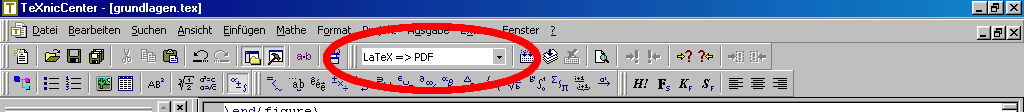
\includegraphics[width=\linewidth]{images/beispiel1_03.png}
	\end{center}
	\caption{Einstellen des Ausgabeformats}
	\label{fig:beispiel1_03}
\end{figure}

Stelle dieses Pulldownmenü auf \enquote{LaTeX => PDF} ein. Ein anderer Weg ist über das Menü: \enquote{Ausgabe} $\Rightarrow$ \enquote{Aktives Ausgabeprofil wählen...}.

\subsection{Speichern und Kompilieren}
\index{Speichern}\index{Kompilieren}

Speichere die Datei jetzt mit \enquote{Ctrl+S} oder über das Menü \enquote{Datei} $\Rightarrow$ \enquote{Speichern} oder durch einen Klick auf das Diskettensymbol in der Symbolleiste.

Jetzt kannst du den Kompiliervorgang mit der Taste \enquote{F7} starten oder über das Menü \enquote{Ausgabe} $\Rightarrow$ \enquote{Projekt compilieren} oder auch über die Symbolleiste.

Im Statusbereich laufen jetzt diverse Meldungen vorbei. Nach einigen Sekunden oder Minuten, je nachdem, wie schnell dein Computer ist, ist der Kompiliervorgang vorbei. Im Statusfenster siehst du z.\,B. folgende Ausgabe:
\begin{lstlisting}
LaTeX-Ergebnis: 0 Fehler, 1 Warnung(en), 0 zu volle/leere Box(en), 1 Seite(n)
\end{lstlisting}

Es sollten beim Kompiliervorgang keine Fehler aufgetreten sein. Hast du trotzdem Fehler, kontrollierst du am besten noch einmal deinen Text. Vielleicht haben sich ja Tippfehler eingeschlichen.

Mit der Taste \enquote{F9} springst du von einem Fehler zum nächsten. Dabei springt der Cursor an die Stelle in deinem Dokument, an welcher der Fehler \emph{vermutet} wird. Natürlich kann sich der Fehler auch einige Zeilen davor oder danach befinden.

Sind alle Fehler behoben, kannst du mit \enquote{F5} oder über das Menü \enquote{Ausgabe} $\Rightarrow$ \enquote{Ausgabe betrachten} das fertige Dokument betrachten. Dazu wird der Adobe Reader gestartet und das fertige Dokument angezeigt (siehe dazu \cref{fig:beispiel1_04}).

\begin{figure}[ht]
	\begin{center}
		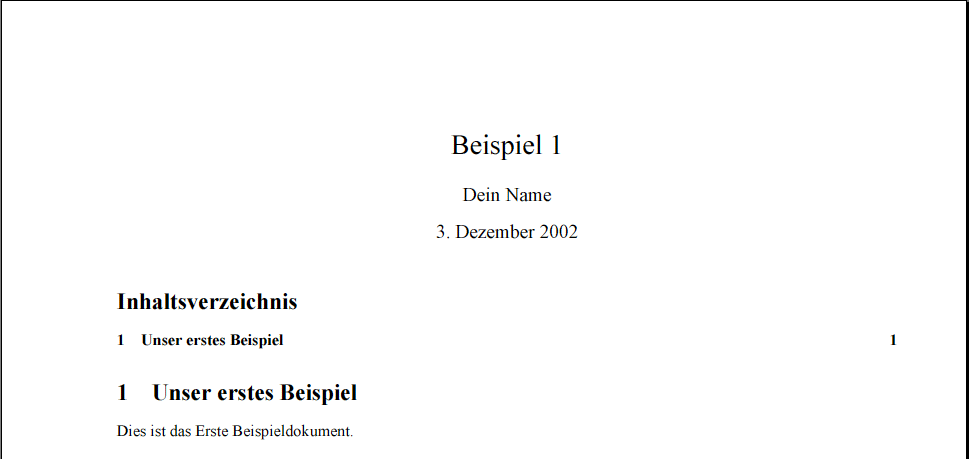
\includegraphics[width=\linewidth]{images/beispiel1_04.png}
	\end{center}
	\caption{Das fertige Beispieldokument}
	\label{fig:beispiel1_04}
\end{figure}

Den Adobe Reader musst du während der Arbeit mit dem TeXnicCenter nicht mehr schließen. Wenn du Änderungen am Dokument machst und dieses übersetzen lässt, kannst du mit \enquote{F5} die Anzeige im bereits geöffneten Adobe Reader einfach auffrischen lassen. Dies geht auch wesentlich schneller, als wenn jedesmal der Adobe Reader gestartet werden müsste.
%TODO: Hier wäre ein Hinweis auf die Vorschau im DVI-Viewer schön -> hier automatischer Refresh

\index{Grundlagen|)}

\section{Sonderzeichen}
\index{Sonderzeichen}\label{Sonderzeichen}

Alle \DMLLaTeX"=Befehle beginnen mit einem \enquote{Backslash}, zudem gibt es einige Sonderzeichen welche du nicht direkt verwenden darfst. Hier das Beispiel eines \DMLLaTeX"=Befehls:
\begin{lstlisting}
	\textbackslash
\end{lstlisting}

Die Sonderzeichen, welche du nicht direkt verwenden darfst, liste ich hier kurz auf. Später erfährst du, wie man diese Sonderzeichen in den Text einbauen kann und welchen Zweck sie haben. Verzichte am Anfang einfach auf diese Zeichen.
\begin{lstlisting}
	% # $ & ~ _ ^ \ { } "
\end{lstlisting}

\section{Kommentare mit \%}
\index{Kommentare}\index{Prozentzeichen}

Das Prozentzeichen (\%) wird für Kommentare innerhalb deiner Datei verwendet. Damit kannst du für dich Anmerkungen machen und Dinge kommentieren. 

Wenn du spezielle Pakete in deinem \DMLLaTeX"=Dokument einbindest, solltest du z.\,B. mit einem kurzen Kommentar beschreiben, was dieses Paket macht.

Falls du ein Prozentzeichen in deinen Text einbauen möchtest, musst du einen Backslash vor das Prozentzeichen setzen.
\begin{lstlisting}
%
% Ein Kommentar
%

Hier mit 100\% ein Prozentzeichen
\end{lstlisting}



